\section{Rotar canales}
\par{El filtro consiste en una rotación de canales en cada píxel, como bien indica su nombre. Y la rotación se da de esta manera:}
\begin{center}
\textbf{R} $\longrightarrow$ \textbf{G}\\
\textbf{G} $\longrightarrow$ \textbf{B}\\
\textbf{B} $\longrightarrow$ \textbf{R}\\
\end{center}

\subsection{Código C}
\par{En el código de C recorremos la matriz iterando sus filas y columnas y modificando un píxel a la vez.
A continuación presentamos su pseudocódigo}

\begin{algorithm}[h!]
\caption{Rotar}
\begin{algorithmic}
  \Function{rotar}{src: *unsigned char, dst: *unsigned char, cols: int, filas: int, srcRowSize: int, dstRowSize: int}
	\State $unsigned~ char~ (*srcMatrix)[srcRowSize] = (unsigned~ char (*)[srcRowSize])~ src$
	\State $unsigned~ char~ (*dstMatrix)[dstRowSize] = (unsigned~ char (*)[dstRowSize])~ dst$
	\For{$f \gets 0~..~filas-1$}
		\For{$c \gets 0~..~cols-1$}
			\State $bgra_t* p_s \gets (bgra_t*)$ \& $srcMatrix[f][c * 4]$
			\State $bgra_t *p_d \gets (bgra_t*)$ \&$dstMatrix[f][c * 4]$
			
			\State $p_d \rightarrow$b $\gets$ $p_s \rightarrow g$
			\State $p_d \rightarrow$g $\gets$ $p_s \rightarrow r$
			\State $p_d \rightarrow$r $\gets$ $p_s \rightarrow b$
			\State $p_d \rightarrow$ a $\gets$ $p_s \rightarrow a$
		\EndFor
	\EndFor
\EndFunction
\end{algorithmic} 
\end{algorithm}
	
\subsection{Código ASM}
\par{El código de ASM recorre la matriz de la misma manera que la recorre el código de C, pero procesa 4 píxeles por iteración.}
\par{Las instrucciones propias de SIMD aceleran mucho el proceso y aportan mejoras considerables incluso al compararlo con un código de ASM sin utilizarlas.}

En cada ciclo se cargan 4 píxeles en xmm0 y se aplica \textbf{pshufb xmm0, xmm3}, donde este es:
\xmmb{$0f$}{$0c$}{$0e$}{$0d$}{$0b$}{$08$}{$0a$}{$09$}{$07$}{$04$}{$06$}{$05$}{$03$}{$00$}{$02$}{$01$}
Luego se guarda en memoria en la imagen destino, se incrementa el contador en 4 (procesamos 4 píxeles) y los respectivos punteros a las imagenes en 16 (4 píxeles ocupan 16 bytes).	
	
	
\subsection{Experimentación}

\subsubsection{Idea}	
\par{Para la experimentación con Rotar notamos la facilidad con la que se codea y procesa el filtro gracias a las instrucciones de SIMD, por ello quisimos ver si, además, generaban alguna optimización sobre un código sin estas herramientas.}
\par{Luego comparamos la eficiencia de ASM contra el código de C y distintas optimizaciones de este.}

\subsubsection{Hipótesis}
\par{La hipótesis que tuvimos sobre la primera idea era que efectivamente íbamos a notar un cambio ya que íbamos a estar procesando la mitad de píxeles por iteración. También suponíamos que iba a ser más complicado manipular los píxeles al no contar con instrucciones como \textbf{shuffle}, \textbf{unpacked}, \textbf{psrlx} y \textbf{psllx}.}
	
\subsubsection{Resultados}
\par{Efectivamente vimos una notoria diferencia entre el código en ASM con y sin SIMD.
Para la implementación del filtro ``sin SIMD'' utilizamos intrucciones de enteros y manipulamos cada pixel por separado, de esta manera nos aseguramos ya que esta implementación sea 4 veces menos eficaz. Para esto implementamos dos códigos distintos, uno cargaba de a dos píxeles, procesaba sus atributos por separado, guardaba la información en un registro de 64 bits y luego escribía a memoria. El otro cargaba cada atributo por separado, es decir leíamos de a byte y luego escribíamos de a byte. Ambos son menos eficientes que el código con instrucciones SSE, pero no se vieron  cambios significantes en el tiempo de ejecución de ambos al compararlos entre sí. En el gráfico a continuación se compra con la segunda implementación explicada, que es ligeramente mejor que la segunda. En particular ambas son entre 6 y 7 veces menos eficaces que el código con SIMD aproximadamente. Atribuímos esto a que no sólo se procesa de a menos píxeles sino que también se lee de esta manera, lo que influye aún más en el tiempo de ejecución. Creemos que la pequeña mejora que implica la segunda implementación se da porque esta si bien lee de a bytes, la caché se encarga de traernos ya los 15 bytes siguientes al que acabamos de leer, y por ende, el siguiente acceso a memoria es casi inmediato. Por ende, tarda practicamente lo mismo en leer dos pixeles cargando de a bytes que leer 2 pixeles cargandolos directamente en un registro de 64 bits. Entonces, en este caso, la diferencia inside en el procesamiento, la primer implementación utiliza shifts, los cuales realentizan el proceso, mientras que la segunda simplemente escribe en memoria, sin realizar ningun proceso sobre la información cargada.\\
\medskip
\textbf{¿Por qué esta nueva implementación es 2 veces más eficiente que O3?} \\
Analizamos el código de ASM que genera la implementación de C optimizada y es realmente rebuscada y extensa en comparación. Entendemos que el beneficio que nos significa el set de instrucciones SSE es el hecho de poder procesar en paralelo; es decir que la vectorización es la que implica una mejora de eficacia en el procesamiento de data. En el caso de este filtro el procesamiento es poco o nulo; en el caso de la implementación explicada anteriormente, la cual opera con registros de 8 bits el procesamiento es nulo, el tiempo de ejecución es simplemente el tiempo que se tarda en leer y escribir a memoria. En este caso podemos entender por qué este código es mejor que el O3; ya que la verdadera diferencia que hace SIMD es el procesamiento y en este caso no tenemos, en cambio el ASM generado por la implementación de C optimizado procesa mucho los datos para poder realizar con exito el filtro, lo que genera esta diferencia en el tiempo de ejecución.\\
\medskip
\textbf{Entonces, ¿por qué nuestro código no es mejor incluso que el ASM con instrucciones SSE?} \\
Esto es porque, si bien en el caso anterior el peso de la diferencia se daba en el procesamiento excesivo de los datos, en nuestro código de ASM esto no sucede, utilizamos una sola instrucción la cual manipula los datos y luego el resto es leer y escribir. Pero procesamos 4 píxeles por vez, y esa es la única diferencia sustancial entre dichas implementaciones de ASM.
}
\newpage
\par{A continuación adjuntamos un gráfico en el que se puede apreciar dicha diferencia.}
	
\begin{figure}[H]
\centering
\captionsetup{justification=centering}
	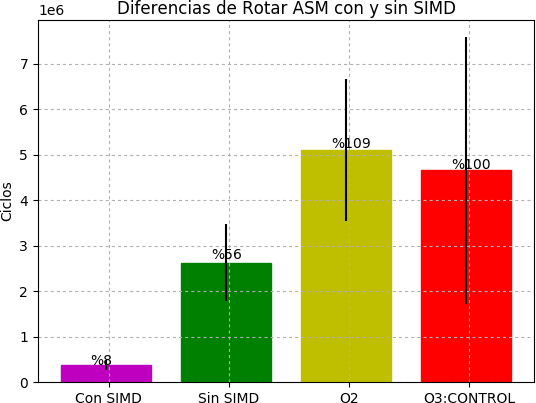
\includegraphics[width = 15 cm, height = 10 cm]{imagenes/RotarSinSIMD.png}
\caption[center]{Gráfico que compara el tiempo de ejecución de las implementaciones con y sin el uso de instrucciones SSE, y también con optimizaciones de la implementación en C.}
\end{figure}

\par{A continuación mostramos un gráfico (armado de igual manera que el anterior) donde mostramos los tiempos de ejecución del filtro implementado en ASM y en C con distintas optimizaciones.}
	
\begin{figure}[H]
\centering
\captionsetup{justification=centering}
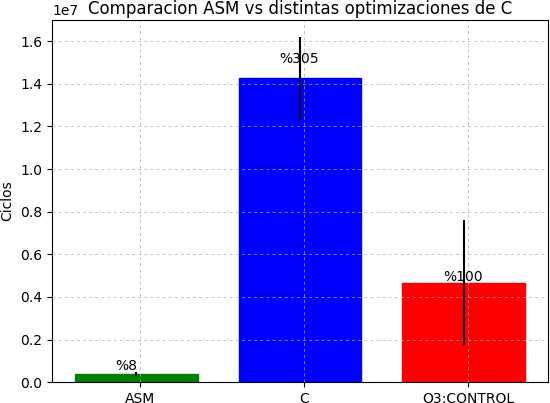
\includegraphics[width = 12 cm, height = 7 cm]{imagenes/ASMvsCRotar.png}
\caption[center]{Diferencias en cantidad de ciclos para la ejecución del filtro con la implementación en ASM y la de C con sus optimizaciones.}
\end{figure}